\begin{center}
    \begin{minipage}{0.45\textwidth}
        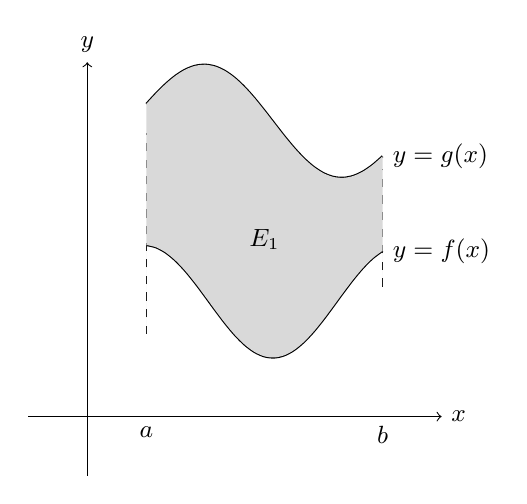
\begin{tikzpicture}[scale=1.5]
            % Ejes
            \draw[->] (-0.5,0) -- (3,0) node[right] {\small $x$};
            \draw[->] (0,-0.5) -- (0,3) node[above] {\small $y$};

            % Curvas más variadas
            \draw[thick, domain=0.5:2.5, smooth, variable=\x] plot ({\x}, {1 + 0.4*sin(3*\x r) + 0.1*cos(2*\x r)}) node[right] {\small $y = f(x)$}; % Ajuste aquí
            \draw[thick, domain=0.5:2.5, smooth, variable=\x] plot ({\x}, {2.5 - 0.3*cos(3*\x r) + 0.2*sin(2*\x r)}) node[right] {\small $y = g(x)$};

            % Líneas verticales en x=a y x=b
            \draw[dashed] (0.5,0.7) -- (0.5,2.4);
            \draw[dashed] (2.5,1.1) -- (2.5,2.1);

            % Etiquetas a y b
            \node[below] at (0.5,0) {\small $a$};
            \node[below] at (2.5,0) {\small $b$};

            % Región sombreada
            \begin{scope}
                \clip (0.5,0.7) -- plot[domain=0.5:2.5, smooth] (\x, {2.5 - 0.3*cos(3*\x r) + 0.2*sin(2*\x r)}) -- (2.5,1.1) -- plot[domain=2.5:0.5, smooth] (\x, {1 + 0.4*sin(3*\x r) + 0.1*cos(2*\x r)}) -- cycle; % Ajuste aquí
                \fill[gray!30] (0,0) rectangle (3,3);
            \end{scope}

            % Etiqueta de la región
            \node at (1.5,1.5) {\small $E_1$};

        \end{tikzpicture}
    \end{minipage}
    \hspace{0.05\textwidth} % Espacio entre las dos figuras
    \begin{minipage}{0.45\textwidth}

        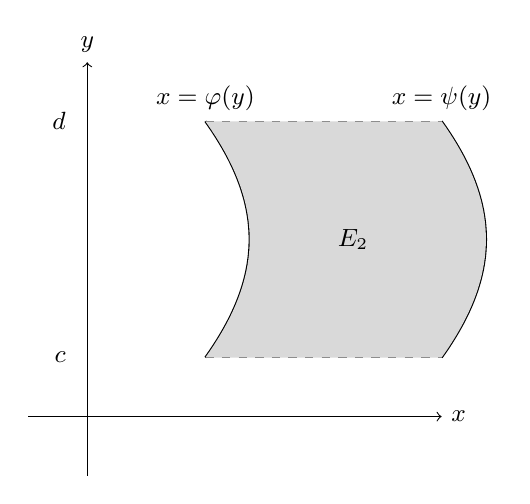
\begin{tikzpicture}[scale=1.5]
            % Ejes de coordenadas con una separación más pequeña
            \draw[->] (-0.5,0) -- (3,0) node[right] {\small $x$};
            \draw[->] (0,-0.5) -- (0,3) node[above] {\small $y$};

            \node[left] at (-0.1,0.5) {\small $c$};  % Etiqueta en y = 0.5
            \node[left] at (-0.1,2.5) {\small $d$};  % Etiqueta en y = 2.5

            % Mover la figura ligeramente a la derecha
            \begin{scope}[shift={(1,0)}]  % Ahora solo 1 unidad a la derecha
                \draw[thick] (0,0.5) .. controls (0.5,1.2) and (0.5,1.8) .. (0,2.5)
                node[above] {\small $x = \varphi(y)$};

                \draw[thick] (2,0.5) .. controls (2.5,1.2) and (2.5,1.8) .. (2,2.5)
                node[above] {\small $x = \psi(y)$};

                % Líneas horizontales
                \draw[dashed] (0,0.5) -- (2,0.5);
                \draw[dashed] (0,2.5) -- (2,2.5);

                % Región sombreada
                \fill[gray!30] (0,0.5) .. controls (0.5,1.2) and (0.5,1.8) .. (0,2.5) --
                (2,2.5) .. controls (2.5,1.8) and (2.5,1.2) .. (2,0.5) -- cycle;

                \node at (1.25,1.5) {\small $E_2$};
            \end{scope}
        \end{tikzpicture}

    \end{minipage}
\end{center}